\documentclass[12pt,letterpaper]{article}
%Preamble:
\input{sl_graphics_preamble.tex}
\graphicspath{{"Figures/"}}
\newenvironment{figenuma}{\begin{inparaenum}[\sffamily a]}{\end{inparaenum}}
\newcommand{\hp}{\hspace{0.5cm}}
\newcommand{\vp}{\vspace{1cm}}
\usepackage[margin=1in]{geometry}
%\usepackage{array}
%\setlength{\extrarowheight}{0.5cm}
%
\begin{document}
\pagestyle{empty}
%
%\begin{flushleft}
%\begin{tabular}{>{\sffamily\bfseries}rc!{\hspace{0.5cm}}c!{\hspace{0.5cm}}c}
%  % after \\: \hline or \cline{col1-col2} \cline{col3-col4} ...
%  a & \aligntop{\includegraphics[height=2cm]{binary.svg}} & \aligntop{\includegraphics[height=2.4cm]{pooled.svg}} & \aligntop{\includegraphics[height=2cm]{multistate.svg}} \\
%  b & \aligntop{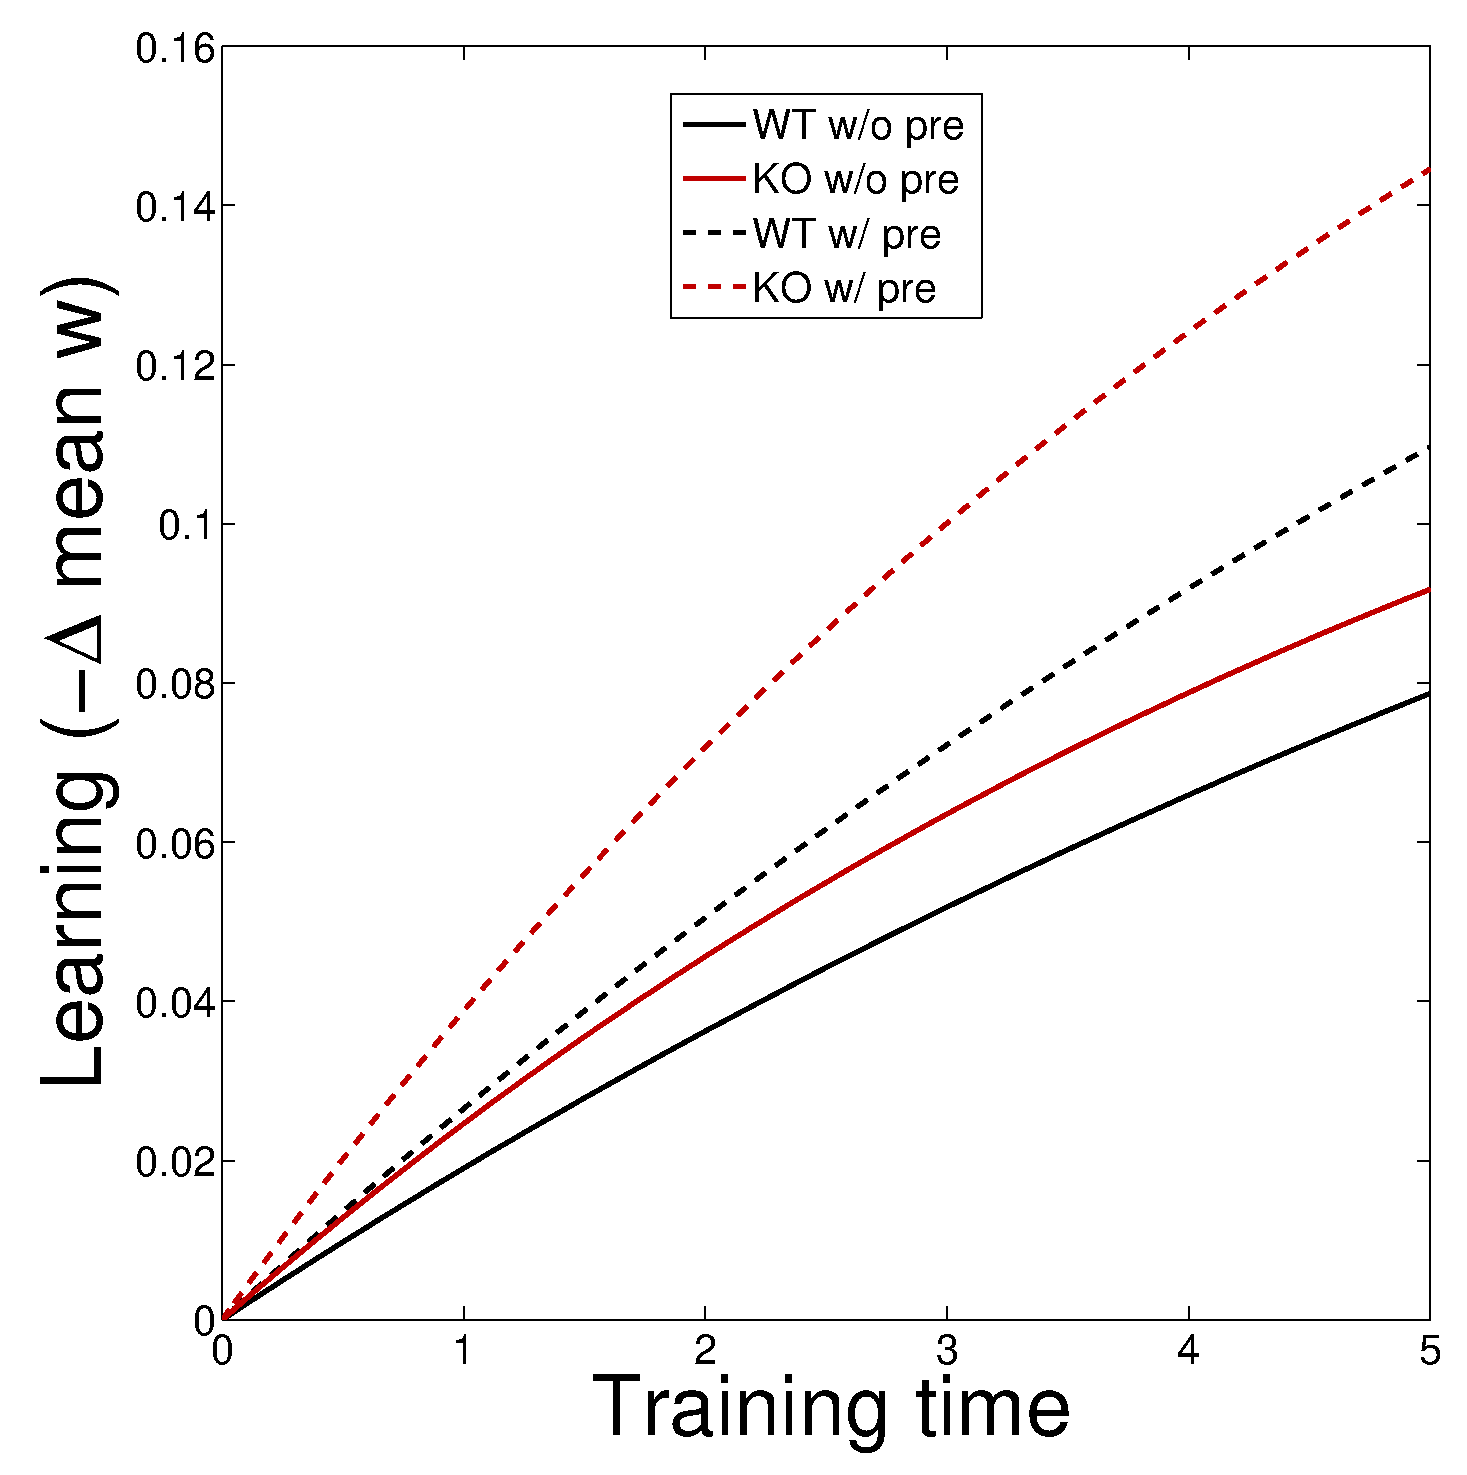
\includegraphics[height=6cm]{binary_learnS.eps}} & \aligntop{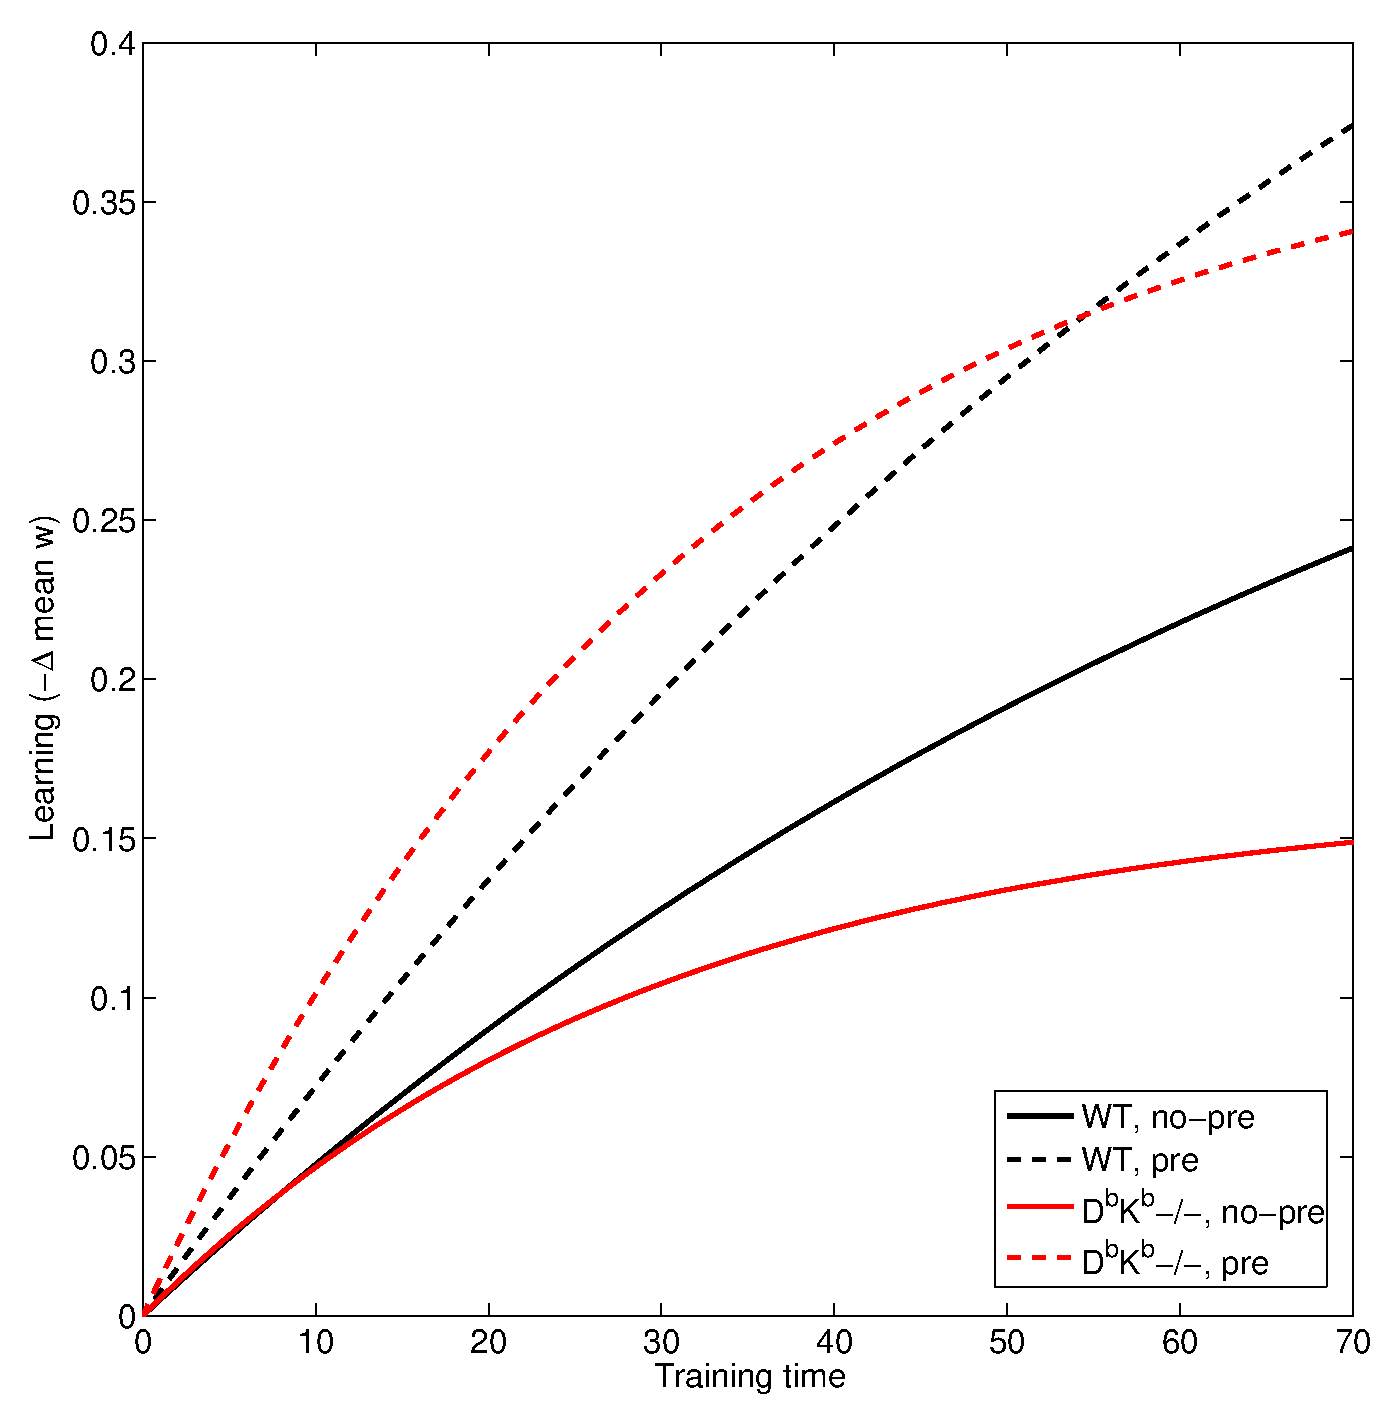
\includegraphics[height=6cm]{pooled_scarce_learnS.eps}} & \aligntop{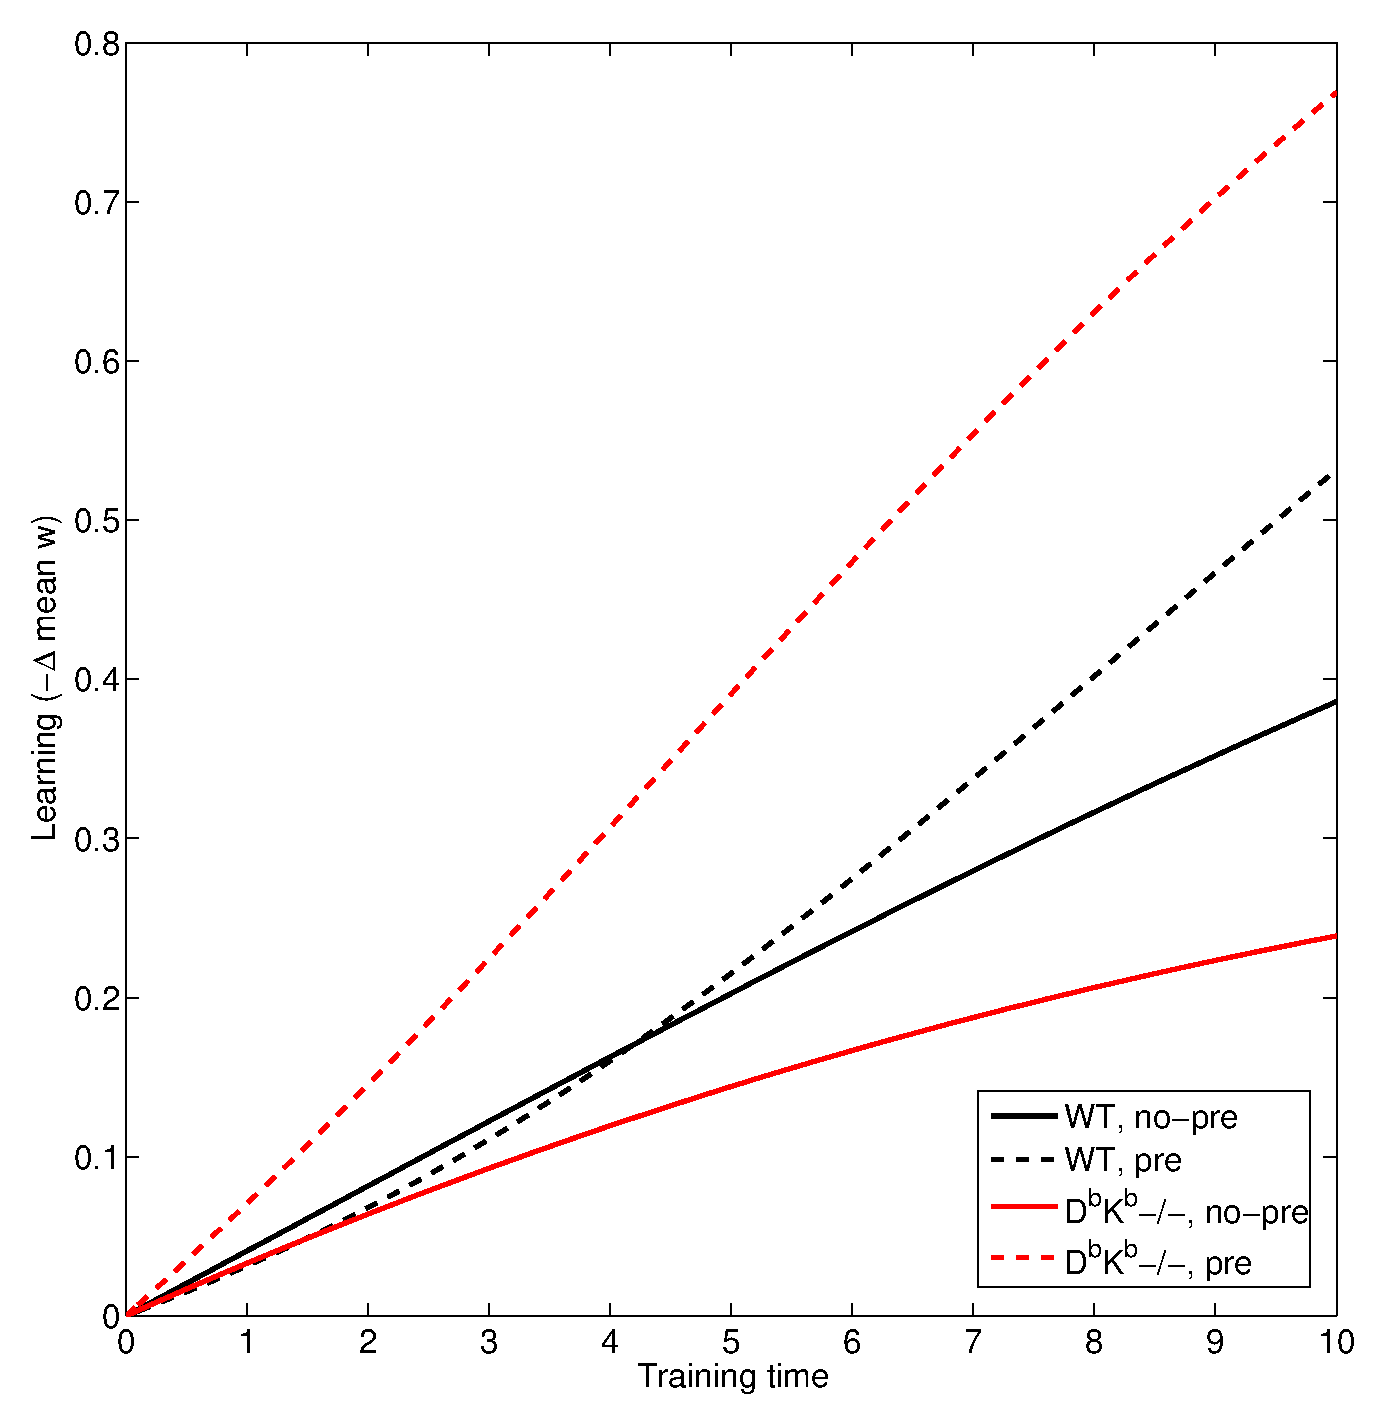
\includegraphics[height=6cm]{multistate_med_learnS.eps}} \\
%  c & \aligntop{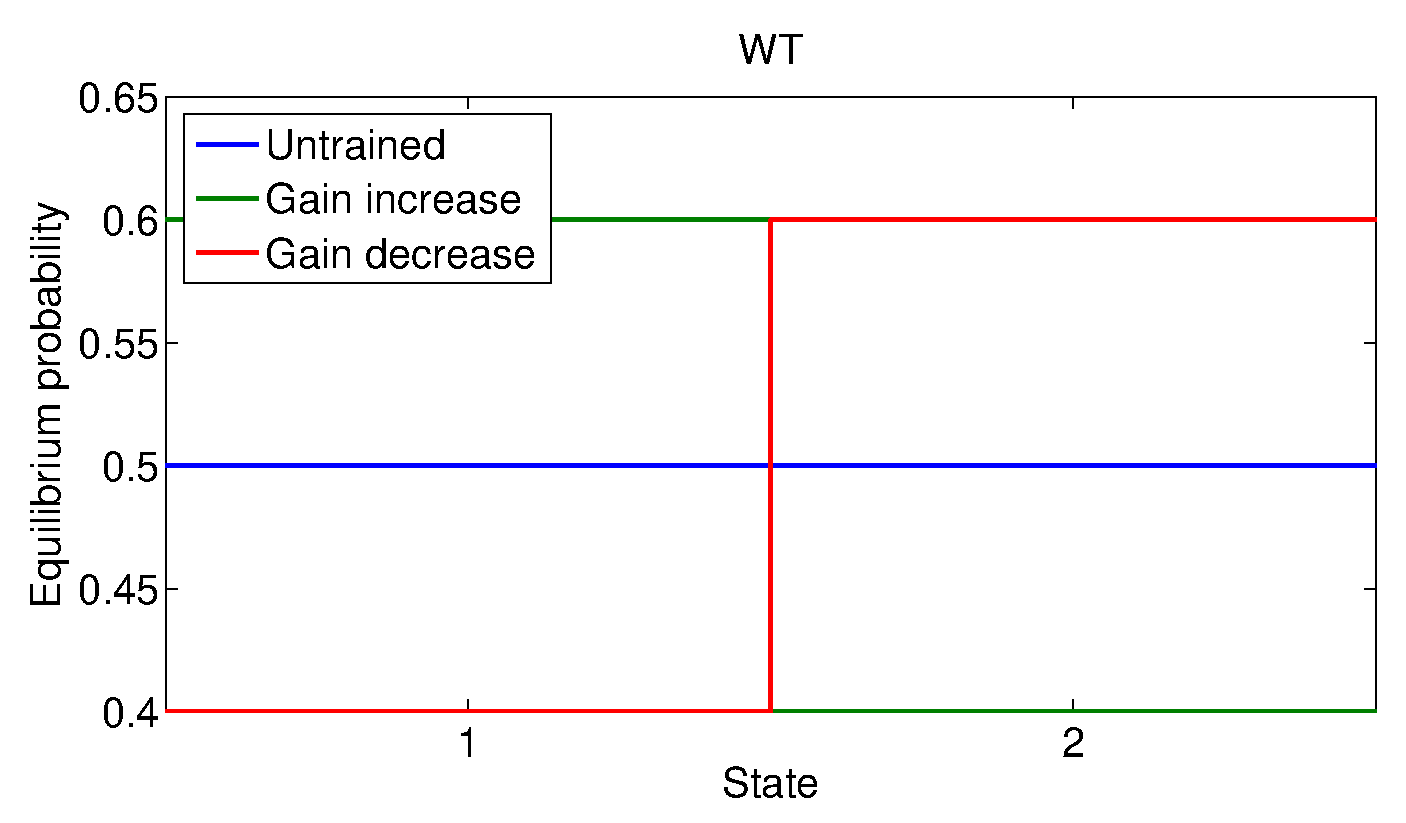
\includegraphics[height=3cm]{binary_eq_WT.eps}} & \aligntop{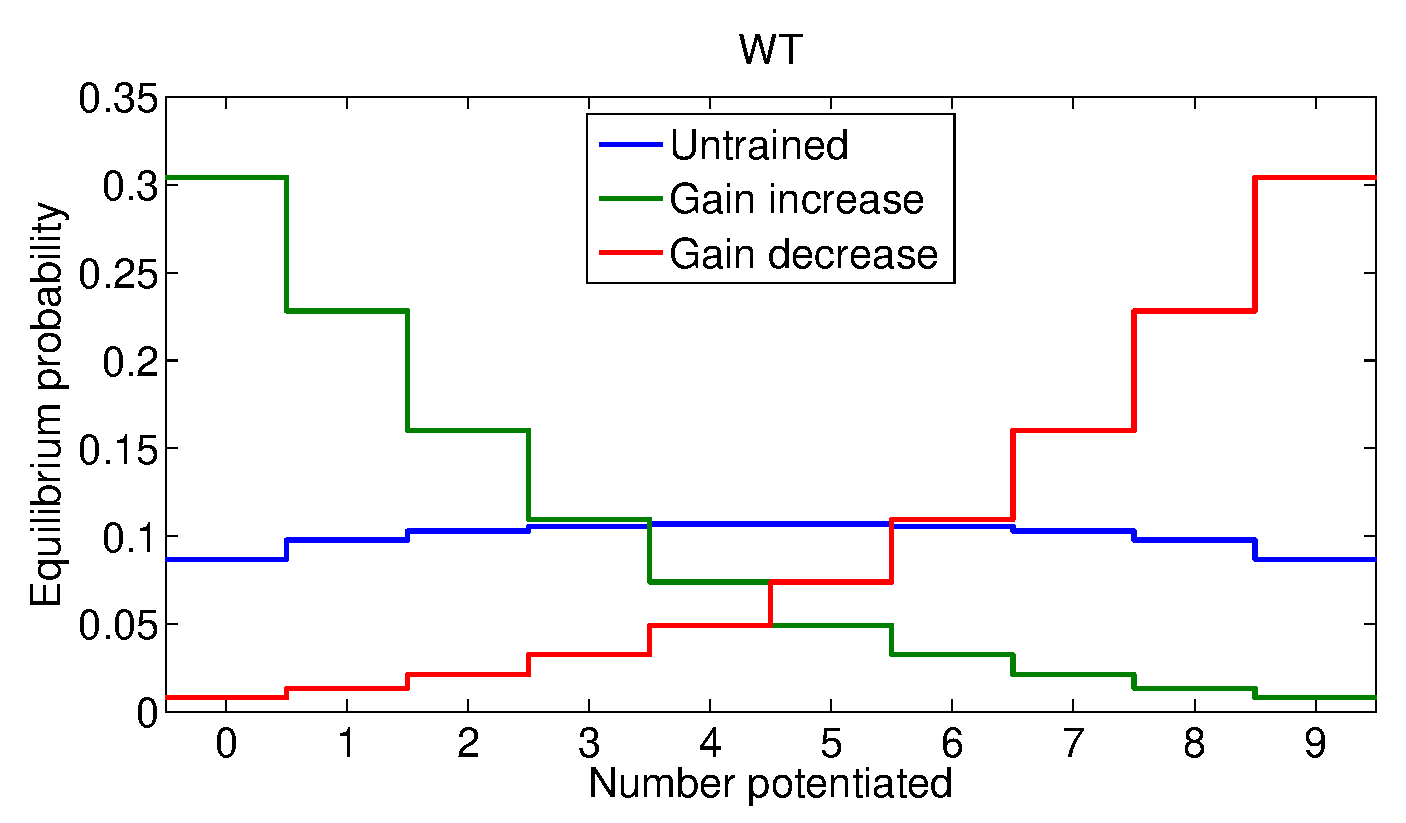
\includegraphics[height=3cm]{pooled_scarce_eq_WT.eps}} & \aligntop{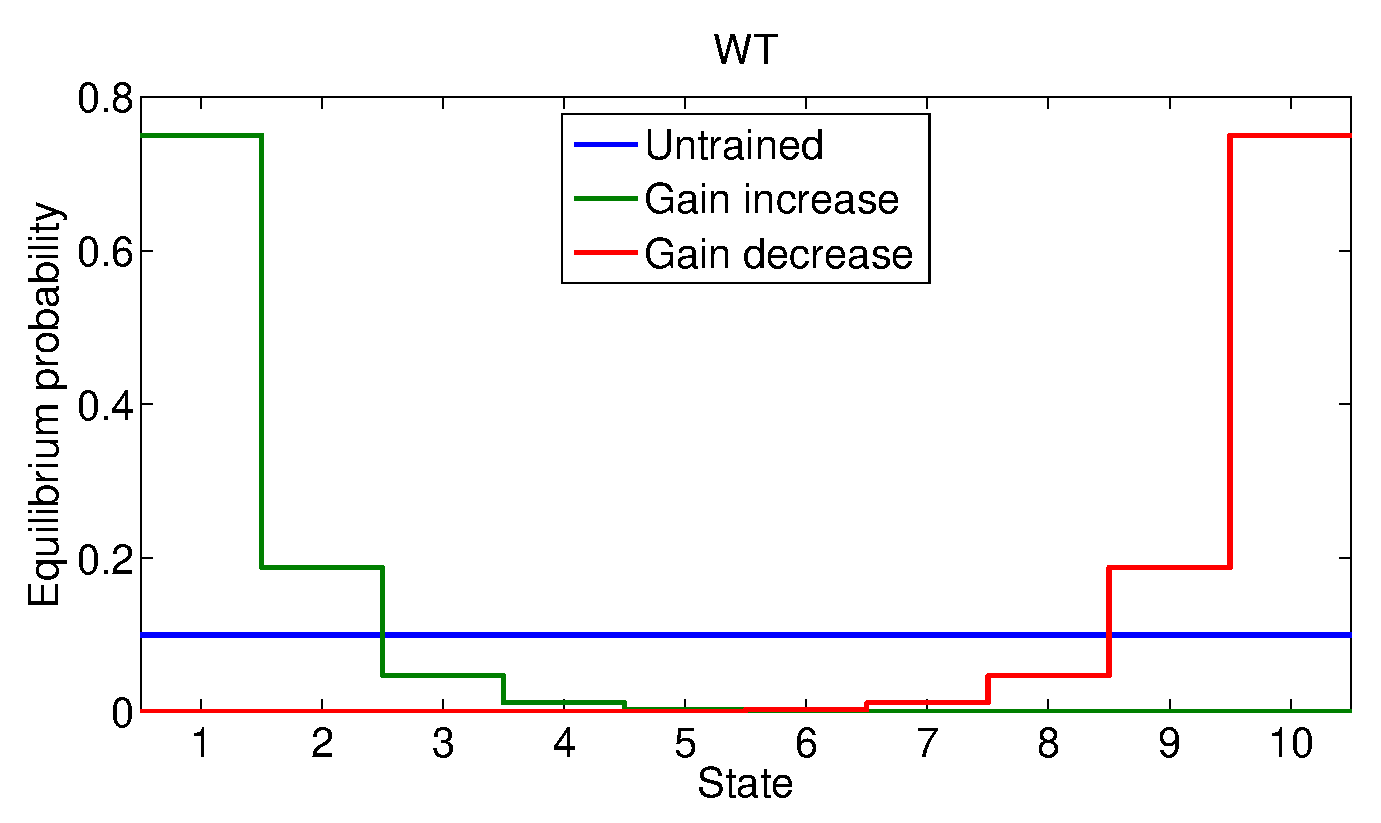
\includegraphics[height=3cm]{multistate_med_eq_WT.eps}} \\
%   & \aligntop{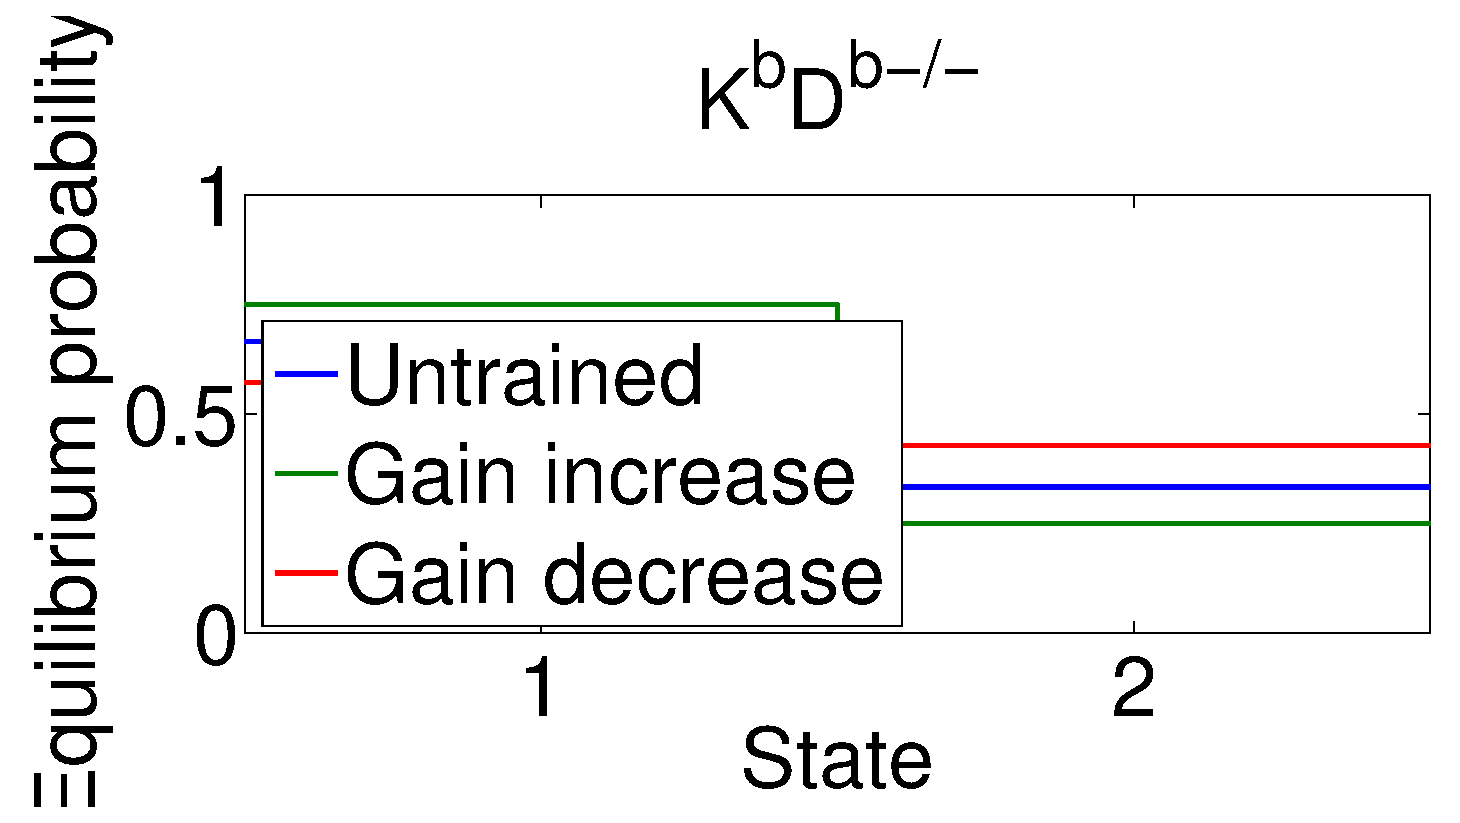
\includegraphics[height=3cm]{binary_eq_KO.eps}} & \aligntop{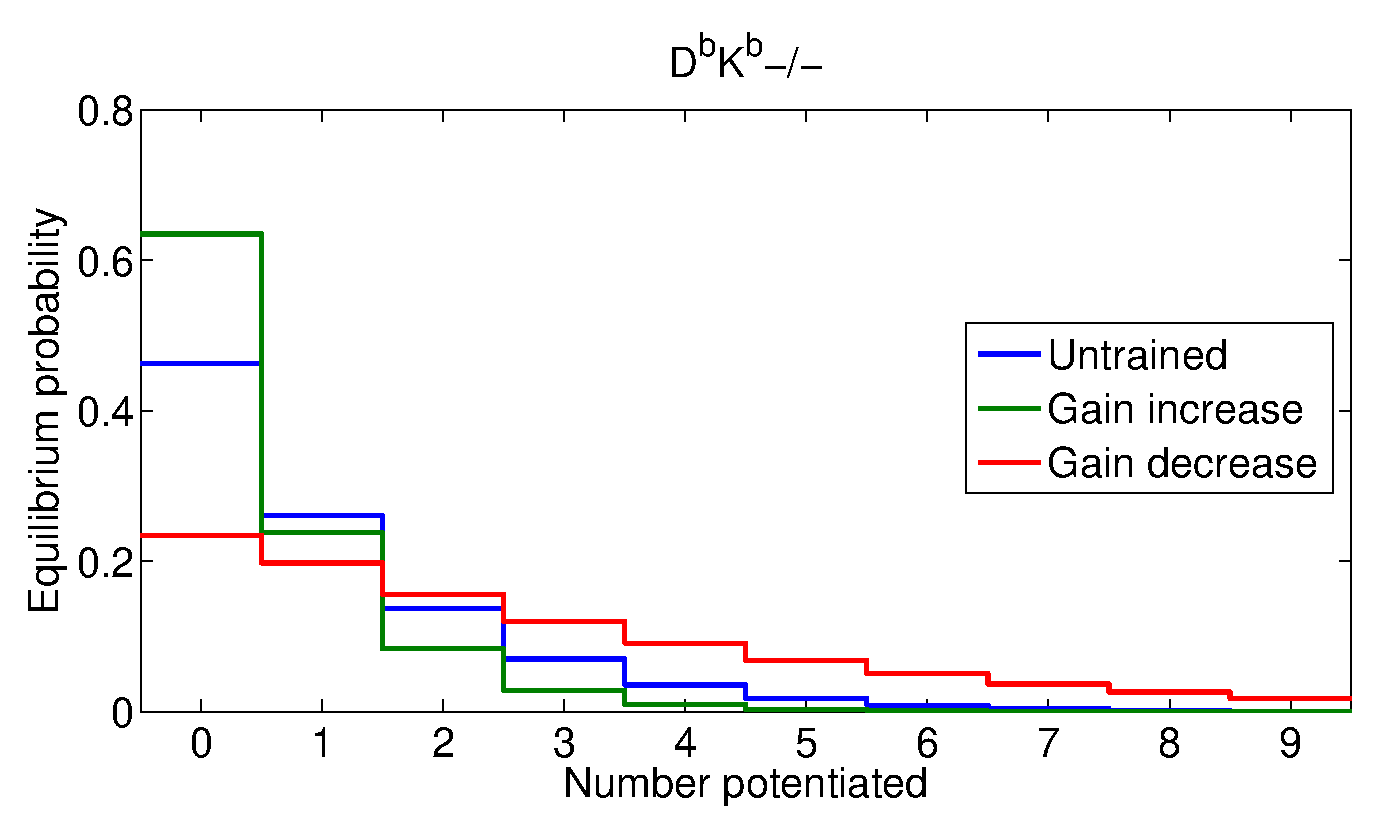
\includegraphics[height=3cm]{pooled_scarce_eq_KO.eps}} & \aligntop{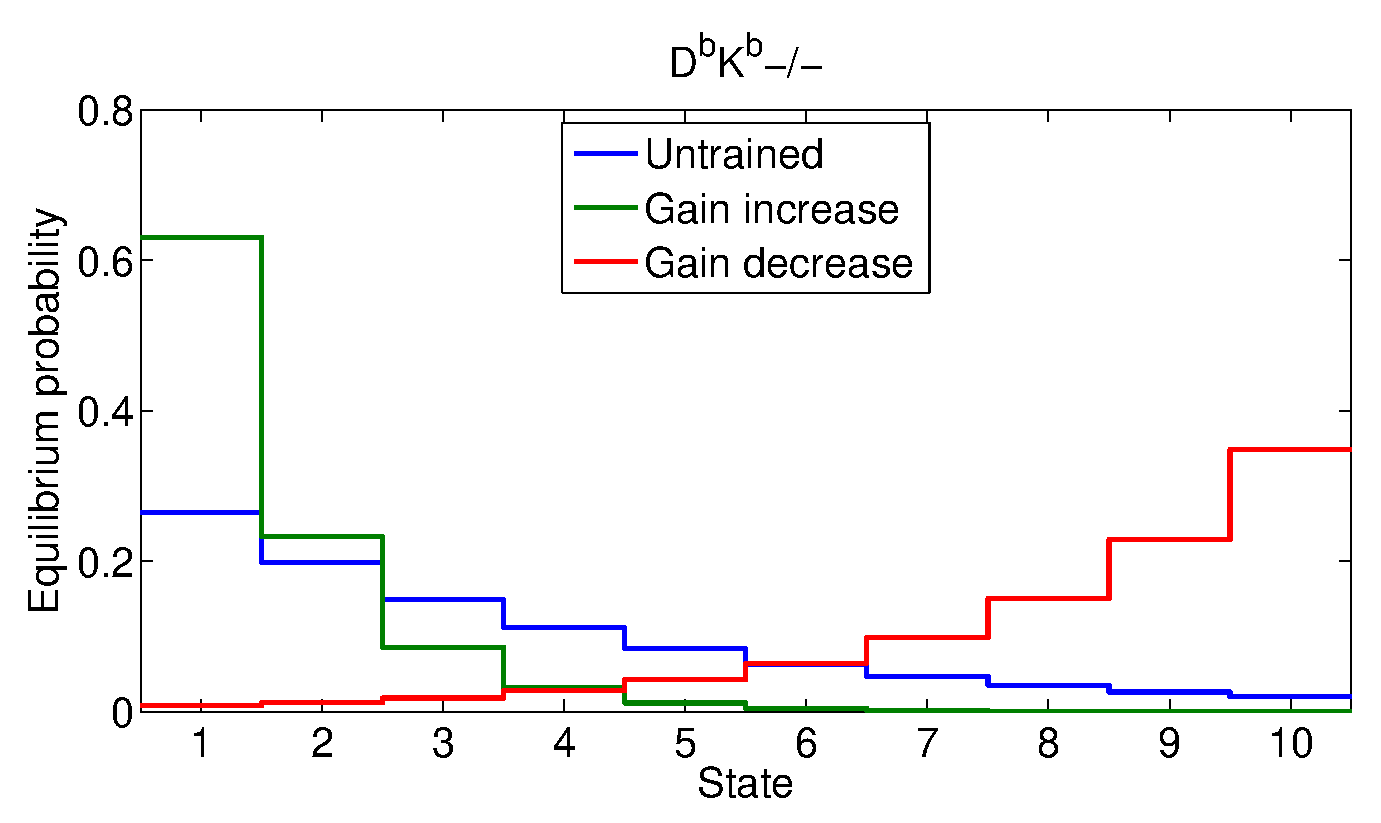
\includegraphics[height=3cm]{multistate_med_eq_KO.eps}} \\
%\end{tabular}
%\end{flushleft}

%
\begin{center}
  \Large{\textsf{Figure 5\_Raymond}}
\end{center}
%
\vp
\begin{flushleft}
\begin{figenuma}
  \item \aligntop{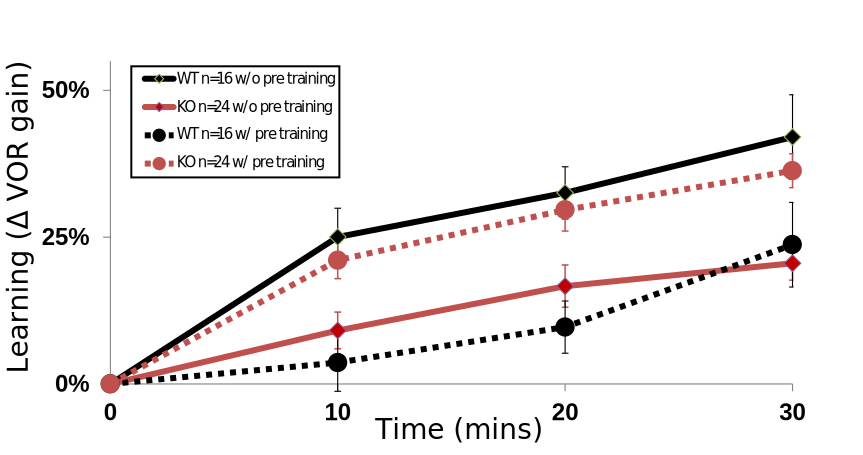
\includegraphics[height=5cm]{data_shifted.svg}}
%  \hp
%  \item \hp\aligntop{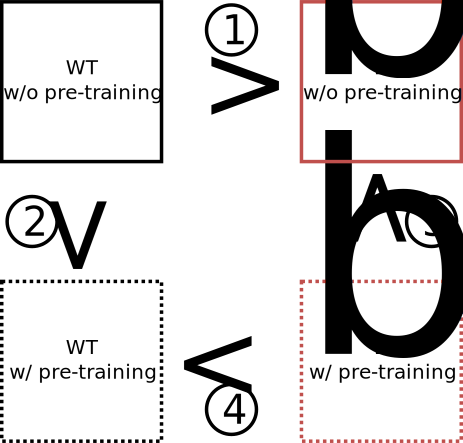
\includegraphics[height=5cm]{comparisons.svg}}
  \\ \vp
  \item \hp\aligntop{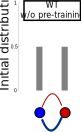
\includegraphics[height=5cm]{binary_bar_wt_wo.svg}}
  \hp
  \item \hp\aligntop{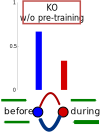
\includegraphics[height=5cm]{binary_bar_ko_wo.svg}}
  \hp
  \item \hp\aligntop{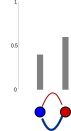
\includegraphics[height=5cm]{binary_bar_wt_w.svg}}
  \hp
  \item \hp\aligntop{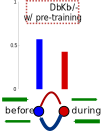
\includegraphics[height=5cm]{binary_bar_ko_w.svg}}
  \\ \vp
  \item \aligntop{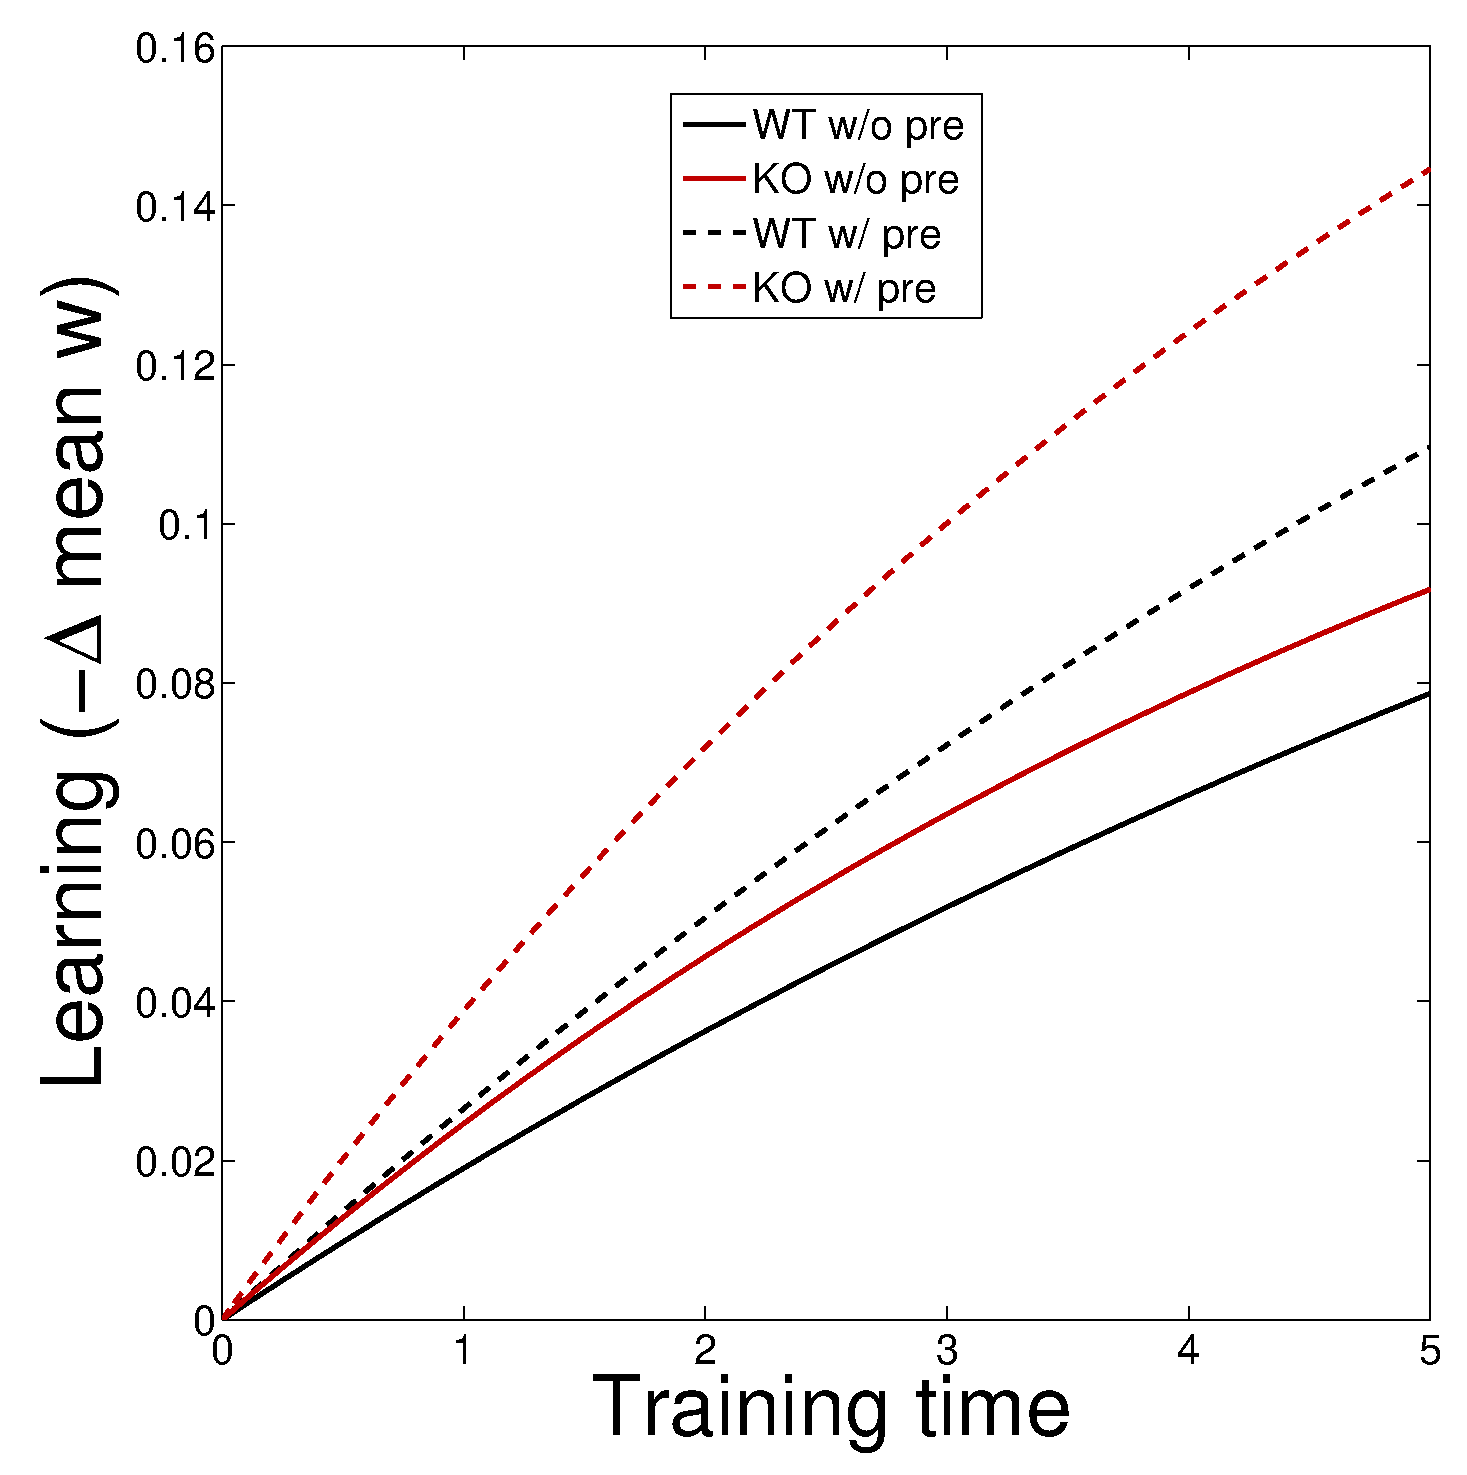
\includegraphics[height=4.5cm]{binary_learnS.eps}}
  \hp
  \item \aligntop{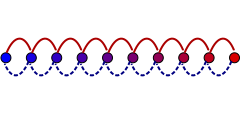
\includegraphics[height=4.5cm]{multistate_lin.svg}}
  \hp
  \item \aligntop{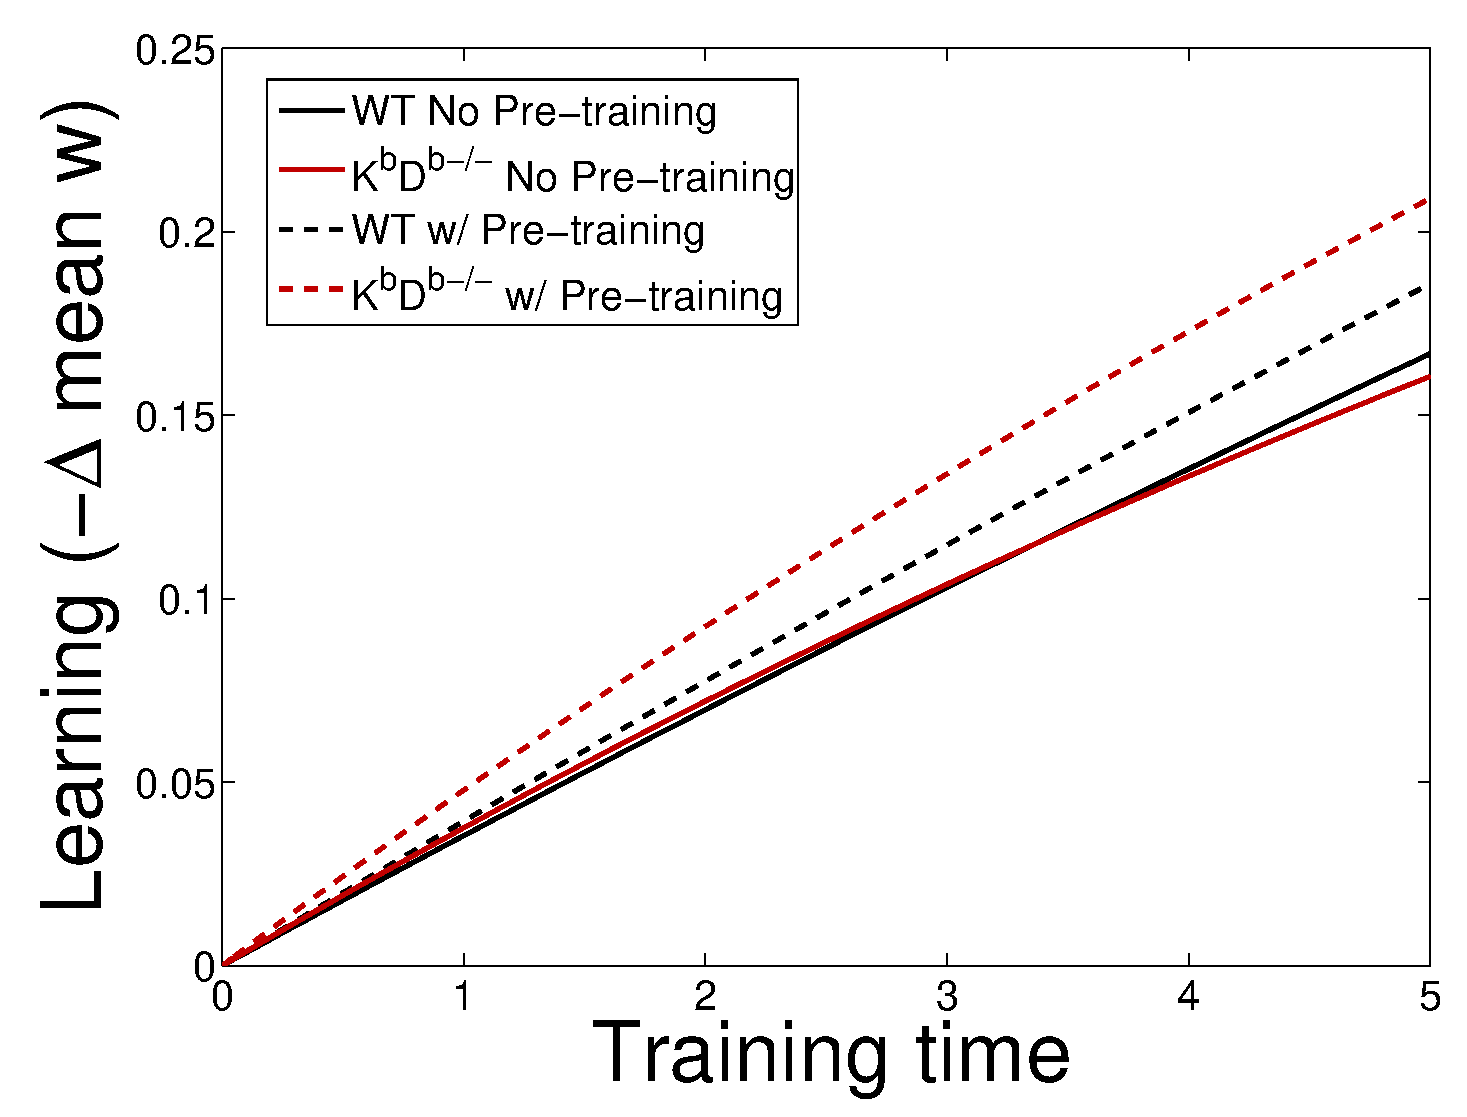
\includegraphics[height=4.5cm]{multistate_lin_learnS.eps}}
\end{figenuma}
\end{flushleft}


\newpage


%
\begin{center}
  \Large{\textsf{Figure 6\_Raymond}}
\end{center}
%
\vp
\begin{flushleft}
\begin{figenuma}
  \item \aligntop{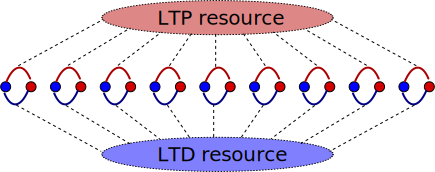
\includegraphics[height=4cm]{pooled_main.svg}}
  \hp
  \item \aligntop{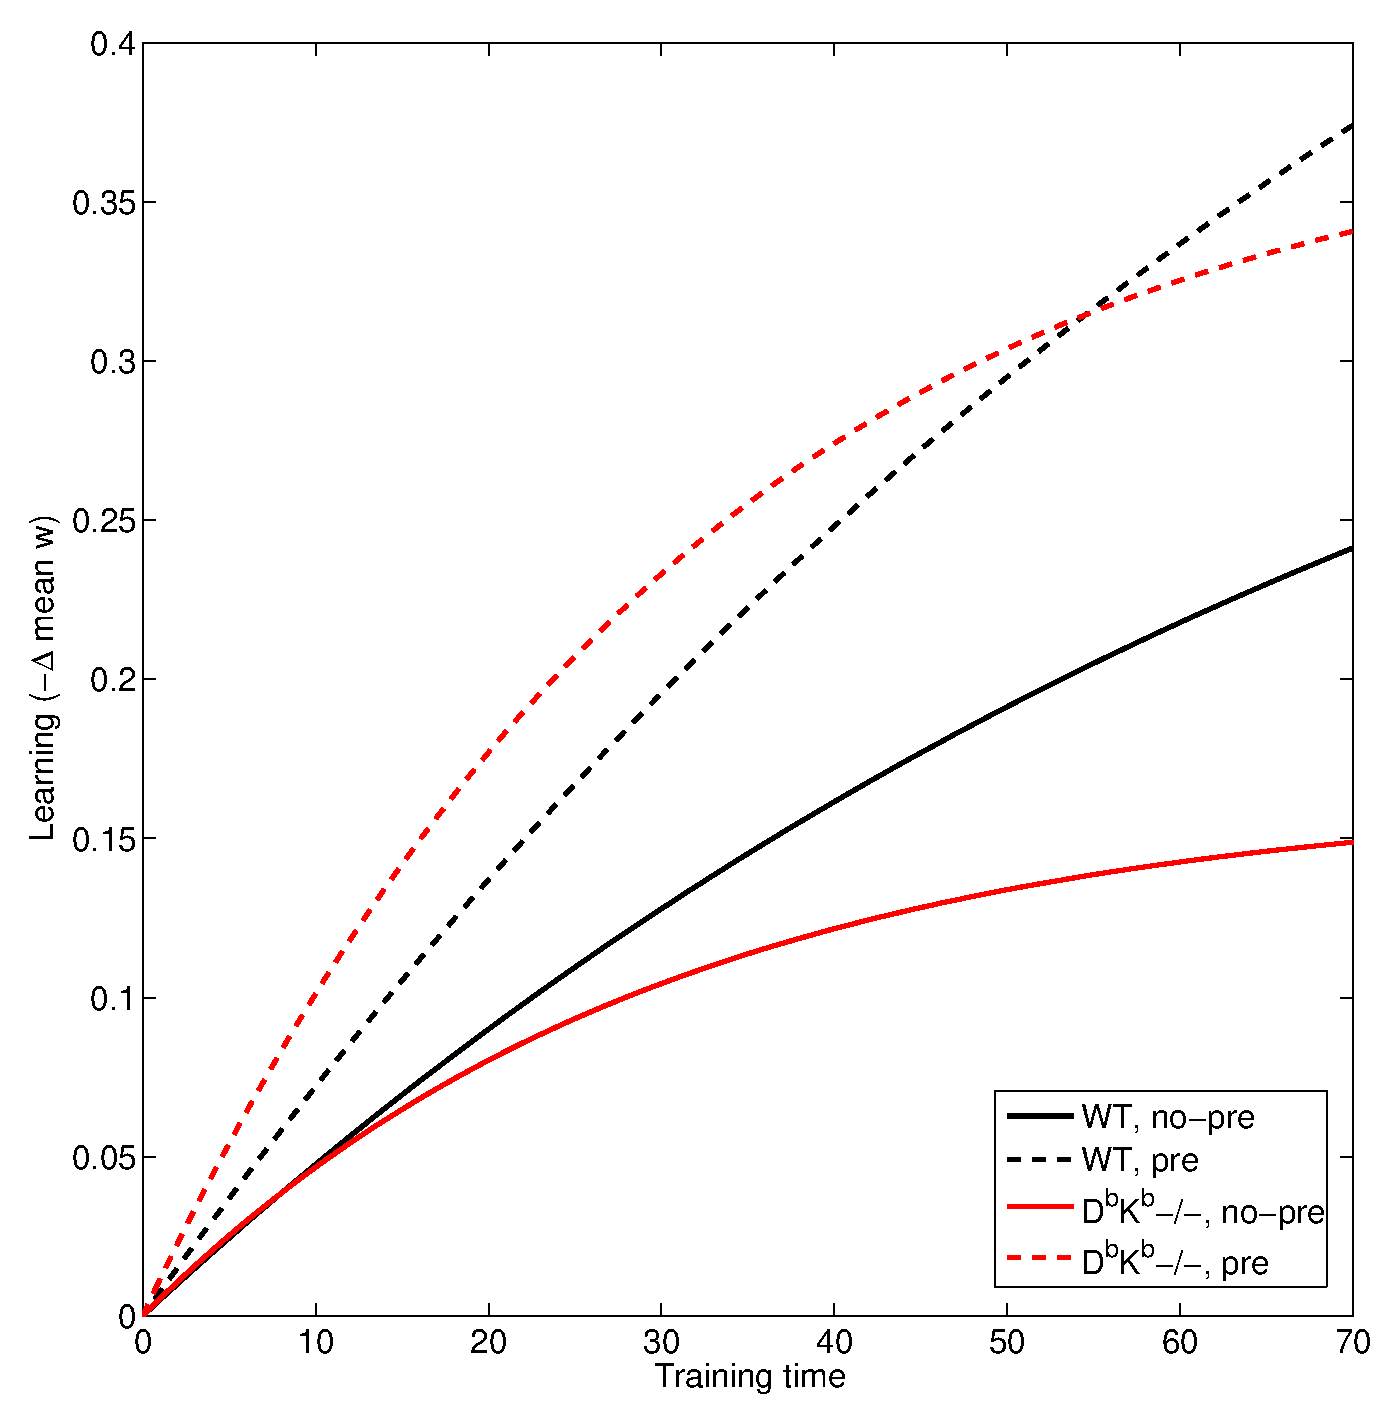
\includegraphics[height=5cm]{pooled_scarce_learnS.eps}}
\end{figenuma}
\end{flushleft}


\newpage


%
\begin{center}
  \Large{\textsf{Figure 7\_Raymond}}
\end{center}
%
\vp
\begin{flushleft}
\begin{figenuma}
  \item \hp\aligntop{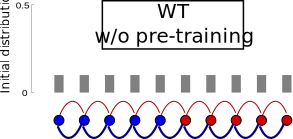
\includegraphics[height=3cm]{multistate_bar_wt_wo.svg}}
  \hp
  \item \hp\aligntop{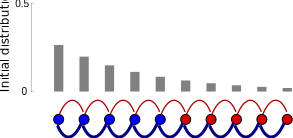
\includegraphics[height=3cm]{multistate_bar_ko_wo.svg}}
  \\ \vp
  \item \hp\aligntop{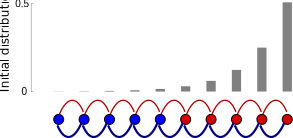
\includegraphics[height=3cm]{multistate_bar_wt_w.svg}}
  \hp
  \item \hp\aligntop{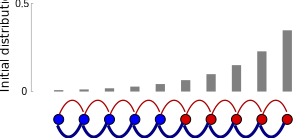
\includegraphics[height=3cm]{multistate_bar_ko_w.svg}}
  \\ \vp
  \item \aligntop{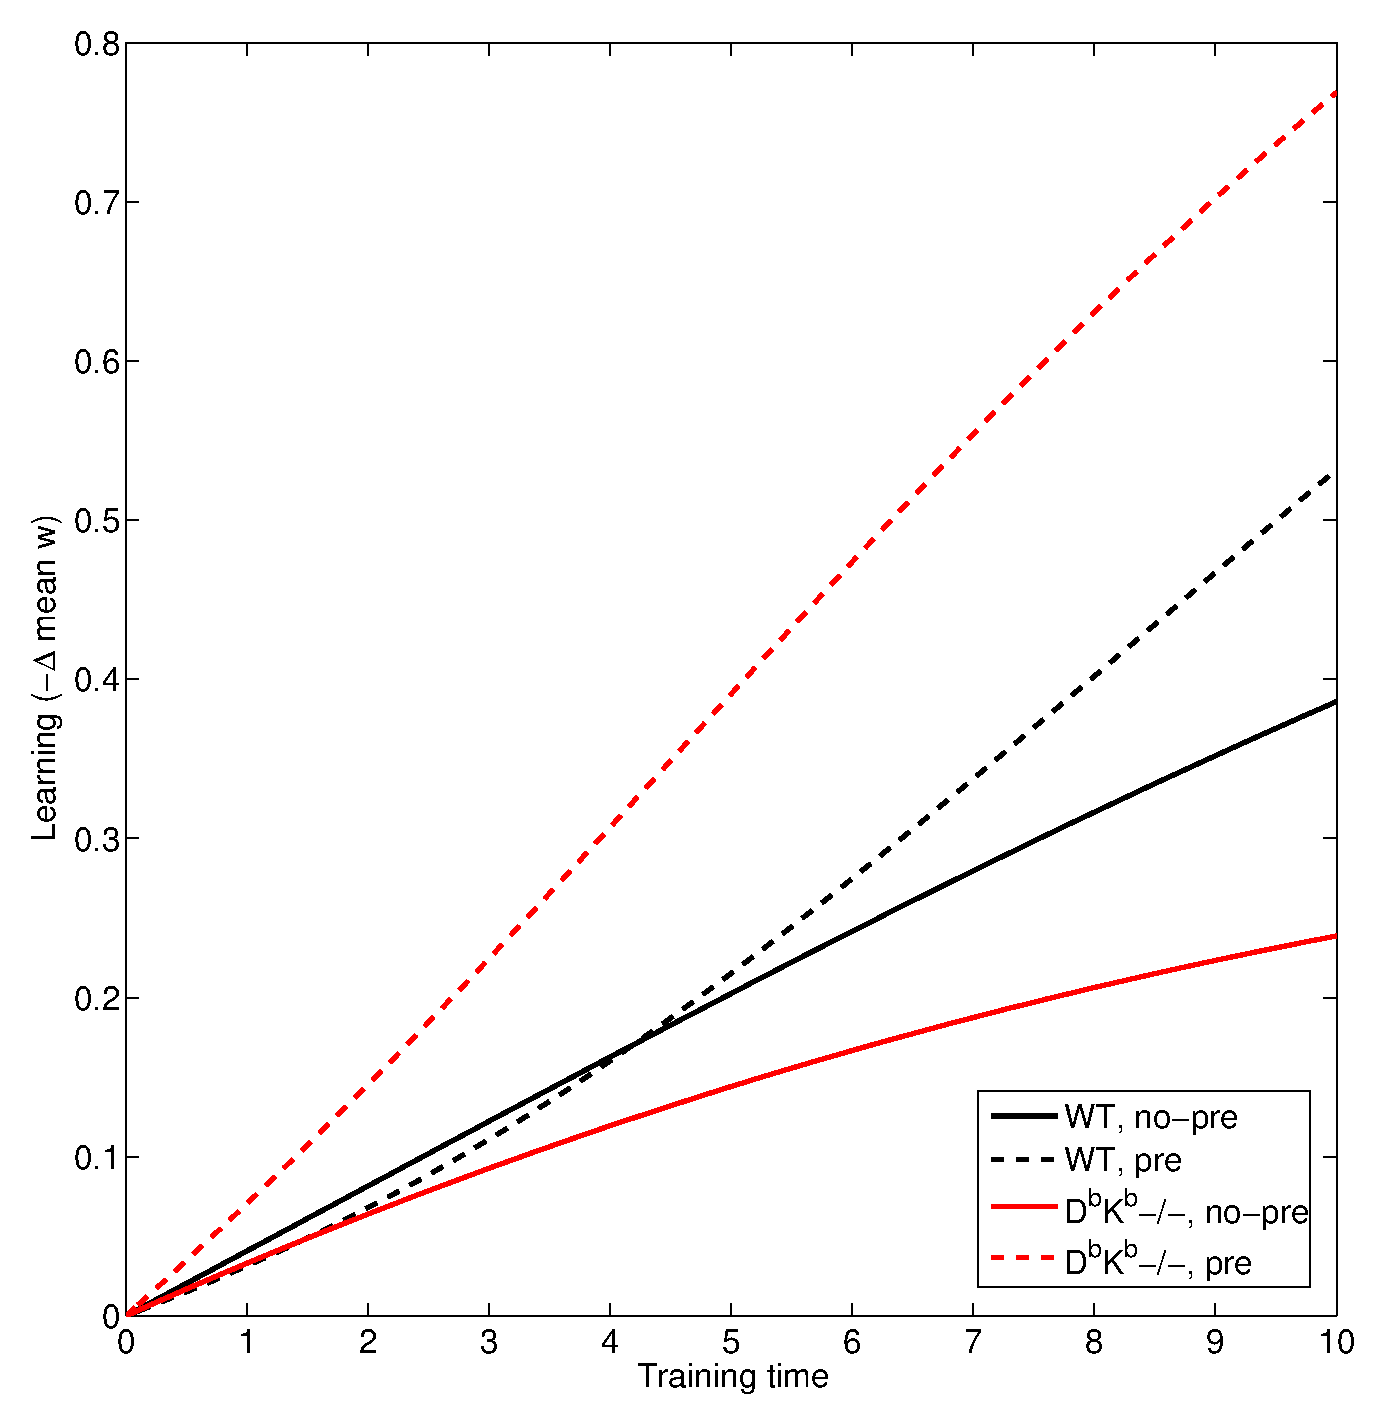
\includegraphics[height=5cm]{multistate_med_learnS.eps}}
  \item \aligntop{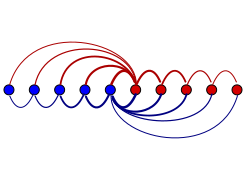
\includegraphics[height=4cm]{cascade_main.svg}}
  \item \aligntop{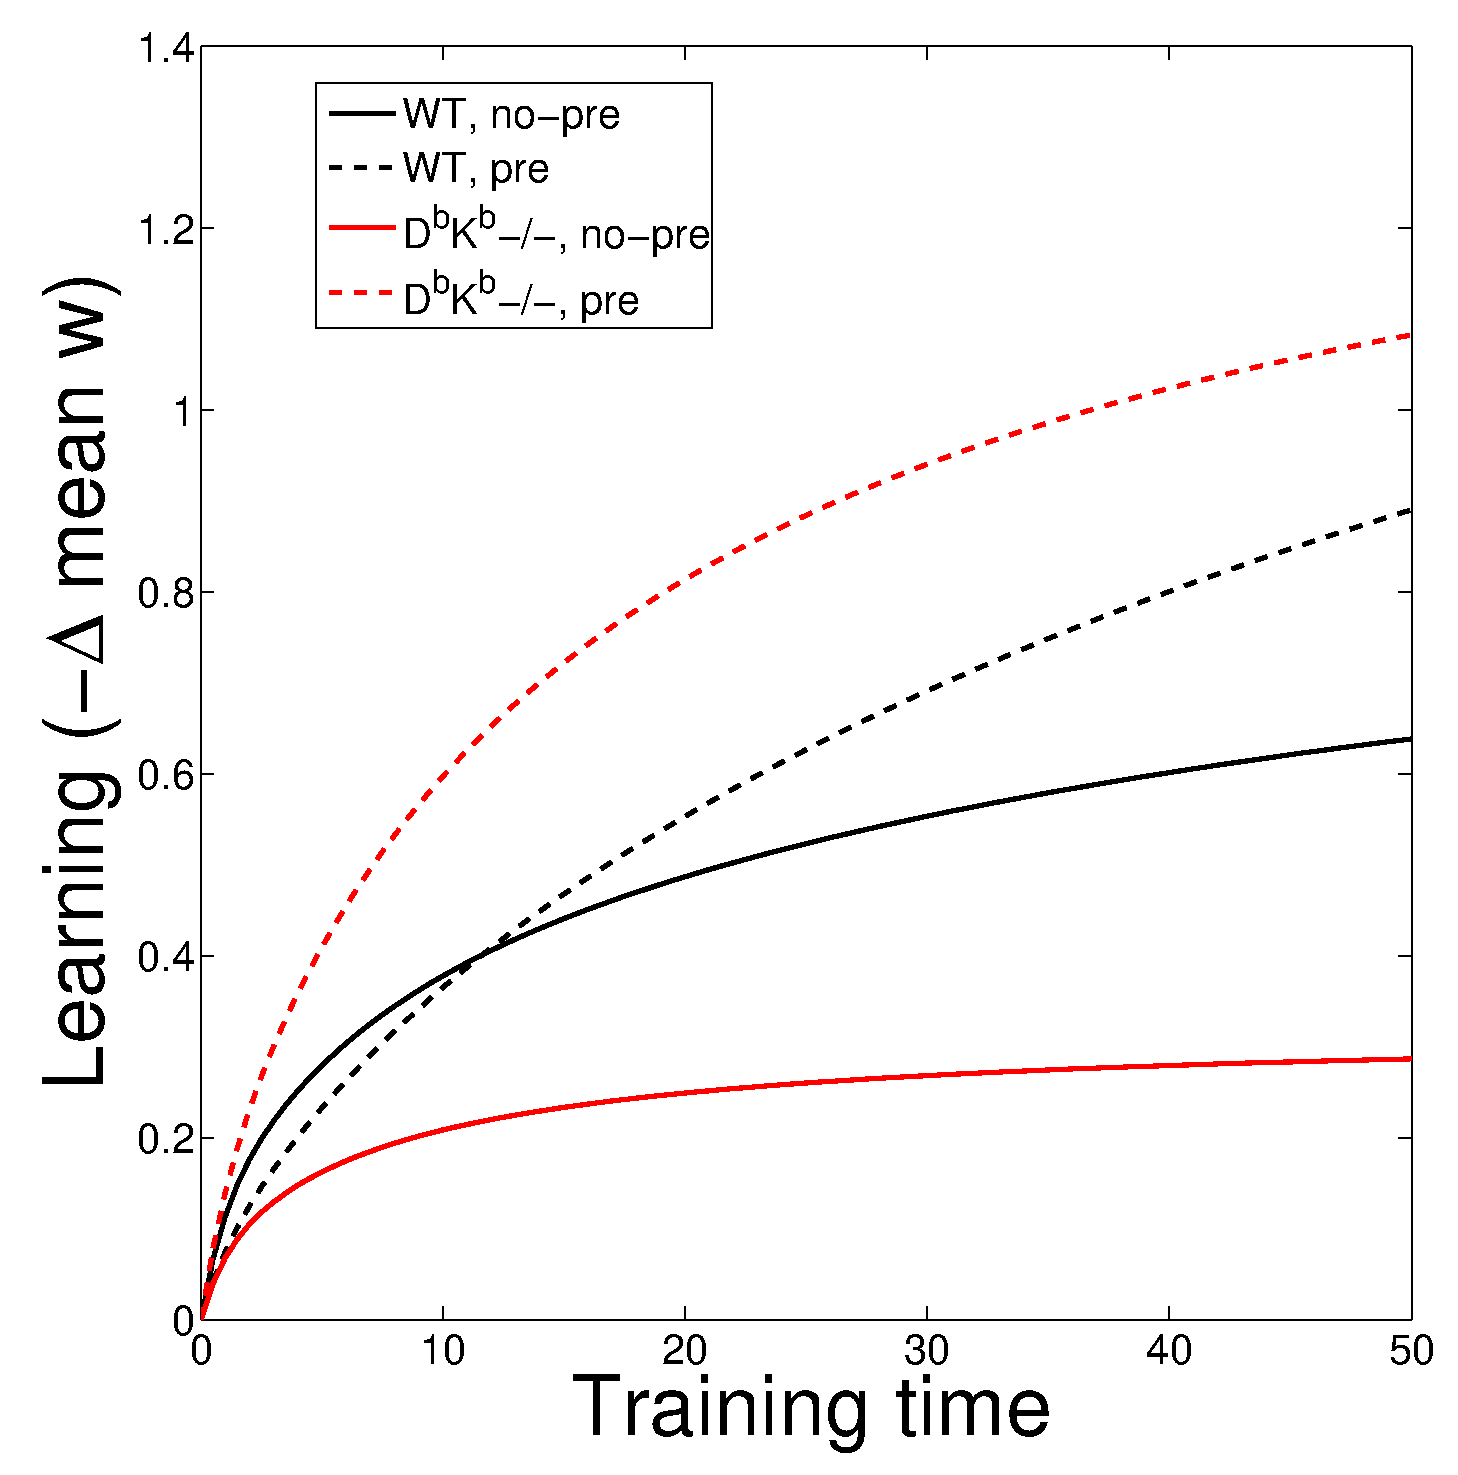
\includegraphics[height=5cm]{cascade_long_learnS.eps}}
\end{figenuma}
\end{flushleft}




\end{document}
